
\documentclass[a4paper,12pt]{report}
%\usepackage[x11names, rgb]{xcolor}
\usepackage[utf8]{inputenc}

\usepackage{makeidx}
\usepackage{longtable}
\usepackage{graphicx}
\usepackage[english]{babel}
\usepackage{babelbib}
\usepackage{verbatim}
\usepackage{verbatimfiles}
\usepackage{alltt}
\usepackage[printonlyused]{acronym}
\usepackage[pdftex,plainpages=false,pdfpagelabels,hyperfootnotes=false]{hyperref}
\usepackage{setspace}
\lefthyphenmin=2
\righthyphenmin=3
\usepackage{afterpage}
\usepackage{csplus}
\usepackage{amsmath}
\usepackage{latexsym}
% \usepackage{thesis}
%\usepackage{pictex}
%\usepackage{specialwords}
\usepackage[binary,squaren]{SIunits}
%\usepackage{hhline}
\usepackage{url}
% \usepackage{dsfont}
% \usepackage{MnSymbol}
\usepackage{listings}
\usepackage{ragbag}
% \usepackage{enumerate}
\raggedbottom

\csplusTitle{ESE CPCC Project}
\csplusAuthor{M. Kleber, C. Krainer, A. Schr\"ocker, B. Zechmeister}
\csplusDate{\today}
\csplusReport{WS 2011/2012}
%\csplusURL{http://www.cs.uni-salzburg.at}
\csplusURL{}
\raggedbottom
\makeindex
\makeglossary


\begin{document}

\setcounter{tocdepth}{3}
\csplusMaketitle
%\onehalfspacing
\begin{abstract}
to be done \ldots
\end{abstract}


\tableofcontents
\setcounter{tocdepth}{3}
\clearpage
\phantomsection
\newpage

\parindent 0pt

%%
%% Introduction
%%

\chapter{Introduction}

Our goal was to build a simulation system that demonstrates information-acquisition-as-a-service
of mobile sensor networks for \ac{CPCC} as proposed in \cite{HotCloud10}.
Based on the JNavigator project \cite{CKrainer2009} our implementation provides
\begin{itemize}
	\item the simulation of physical helicopter swarms,
	\item the simulation of sensors,
	\item the virtual abstraction of autonomous vehicles (virtual vehicles), and
	\item the migration of virtual vehicles among flying physical helicopters (real vehicles).
\end{itemize} 

We consider this project as a first step into the domain of information-acquisition-as-a-service
and therefore allow the following limitations:
\begin{itemize}
	\item Real vehicles follow strict flight plans.
	\item There are no network bandwith limits.
	\item There are no processing power limits.
\end{itemize} 

% leave the following items to future work:

In this project,
\begin{itemize}
	\item we apply \ac{HTTP} as protocol for sensor abstraction and data exchange,
	\item we use Java as programming language,
	\item we implement the software as web applications, and
	\item we utilize Apache Tomcat as web server and servlet container.
\end{itemize} 

This document describes the highlights of the implemented software.
Chapter 2 reveals the implementation details,
chapter 3 describes the project results,
and chapter 4 summarises this paper by depicting proposals for future enhancements.


%%
%% Implementation
%%

\chapter{Implementation}

This chapter presents the implementation of our system.
After outlining the structural elements, it briefly describes the simulation of sensors and explains
configuration parameters. Then, this chapter describes vehicle virtualization, and elaborates on cyber-mobility.

\section{System Overview}

Figure~\ref{fig:SystemOverview} presents an overview of the complete system containing
the ground station and one simulated helicopter referred to as \ac{RV}.

The simulated \ac{RV} mainly comprises an Apache Tomcat web container, which executes a
Pilot web application and an Engine web application.
%
The Pilot web application consists of a model helicopter plant simulator, that is, the MockJAviator,
a flight control system, an auto pilot, and a sensor simulator.
The MockJAviator emulates the helicopter's flight dynamics and \ac{IMU},
the flight control system operates attitude and altitude of the simulated vehicle, 
and the autopilot stirs the simulated vehicle along a \ac{VCL} script defined trajectory.
The sensor simulator supports GPS receivers, belly mounted cameras, thermometers, barometers,
and sonar sensors.
\begin{figure}[h]
	\begin{center}
		{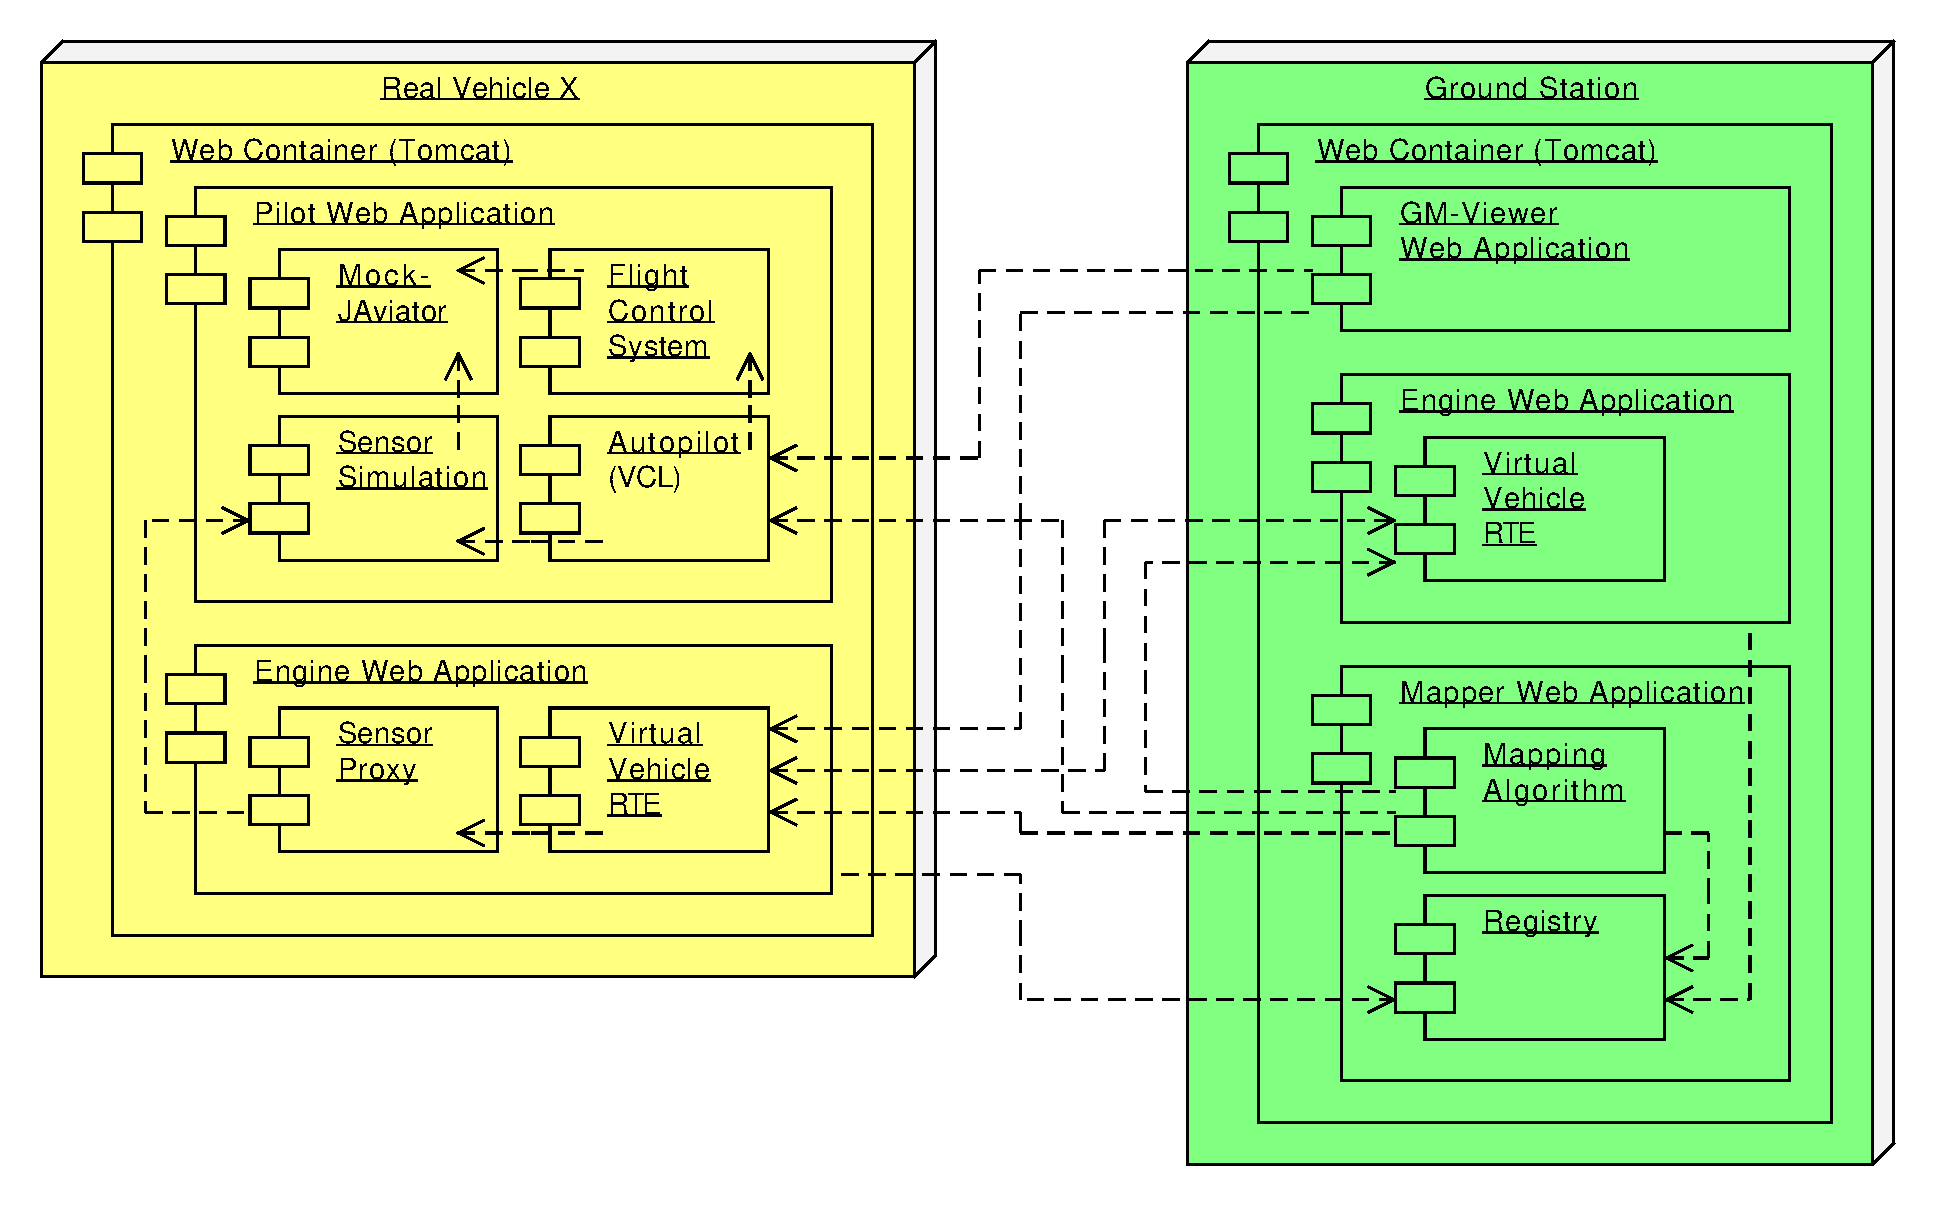
\includegraphics[width=10cm]{SystemOverview.pdf}}
	\end{center}
	\caption{System Overview.\label{fig:SystemOverview}}
\end{figure}
The Engine web application consists of a \ac{VV RTE} and a sensor proxy. The \ac{VV RTE}
handles \ac{VV} execution and the sensor proxy abstracts the access to sensors, as well as
optimizes the network traffic for accessing the sensors.

The ground station executes an Apache Tomcat web container, which runs a Google Maps Viewer
web application, a Engine web application, and a Mapper web application.
%
The Google Maps Viewer web application allows an operator to supervise ongoing missions.
%
The ground station Engine web application provides a \ac{VV RTE} for uploading and downloading \acp{VV}. 
%
Registry and mapping algorithm are the main components of the Mapper web application.
The mapping algorithm assigns \acp{VV} to \acp{RV}, based on fight plans and available sensors.
%
Each Engine web application registers with the Mapper's registry.


\section{Sensor Simulation}
Figure~\ref{fig:SensorSimulation} visualizes the simulation of sensors.
%
The current implementation supports belly mounted cameras, random number generators for emulating thermometers and
barometers, GPS position sensors, and sonar sensors.

 
\begin{figure}[h]
	\begin{center}
		{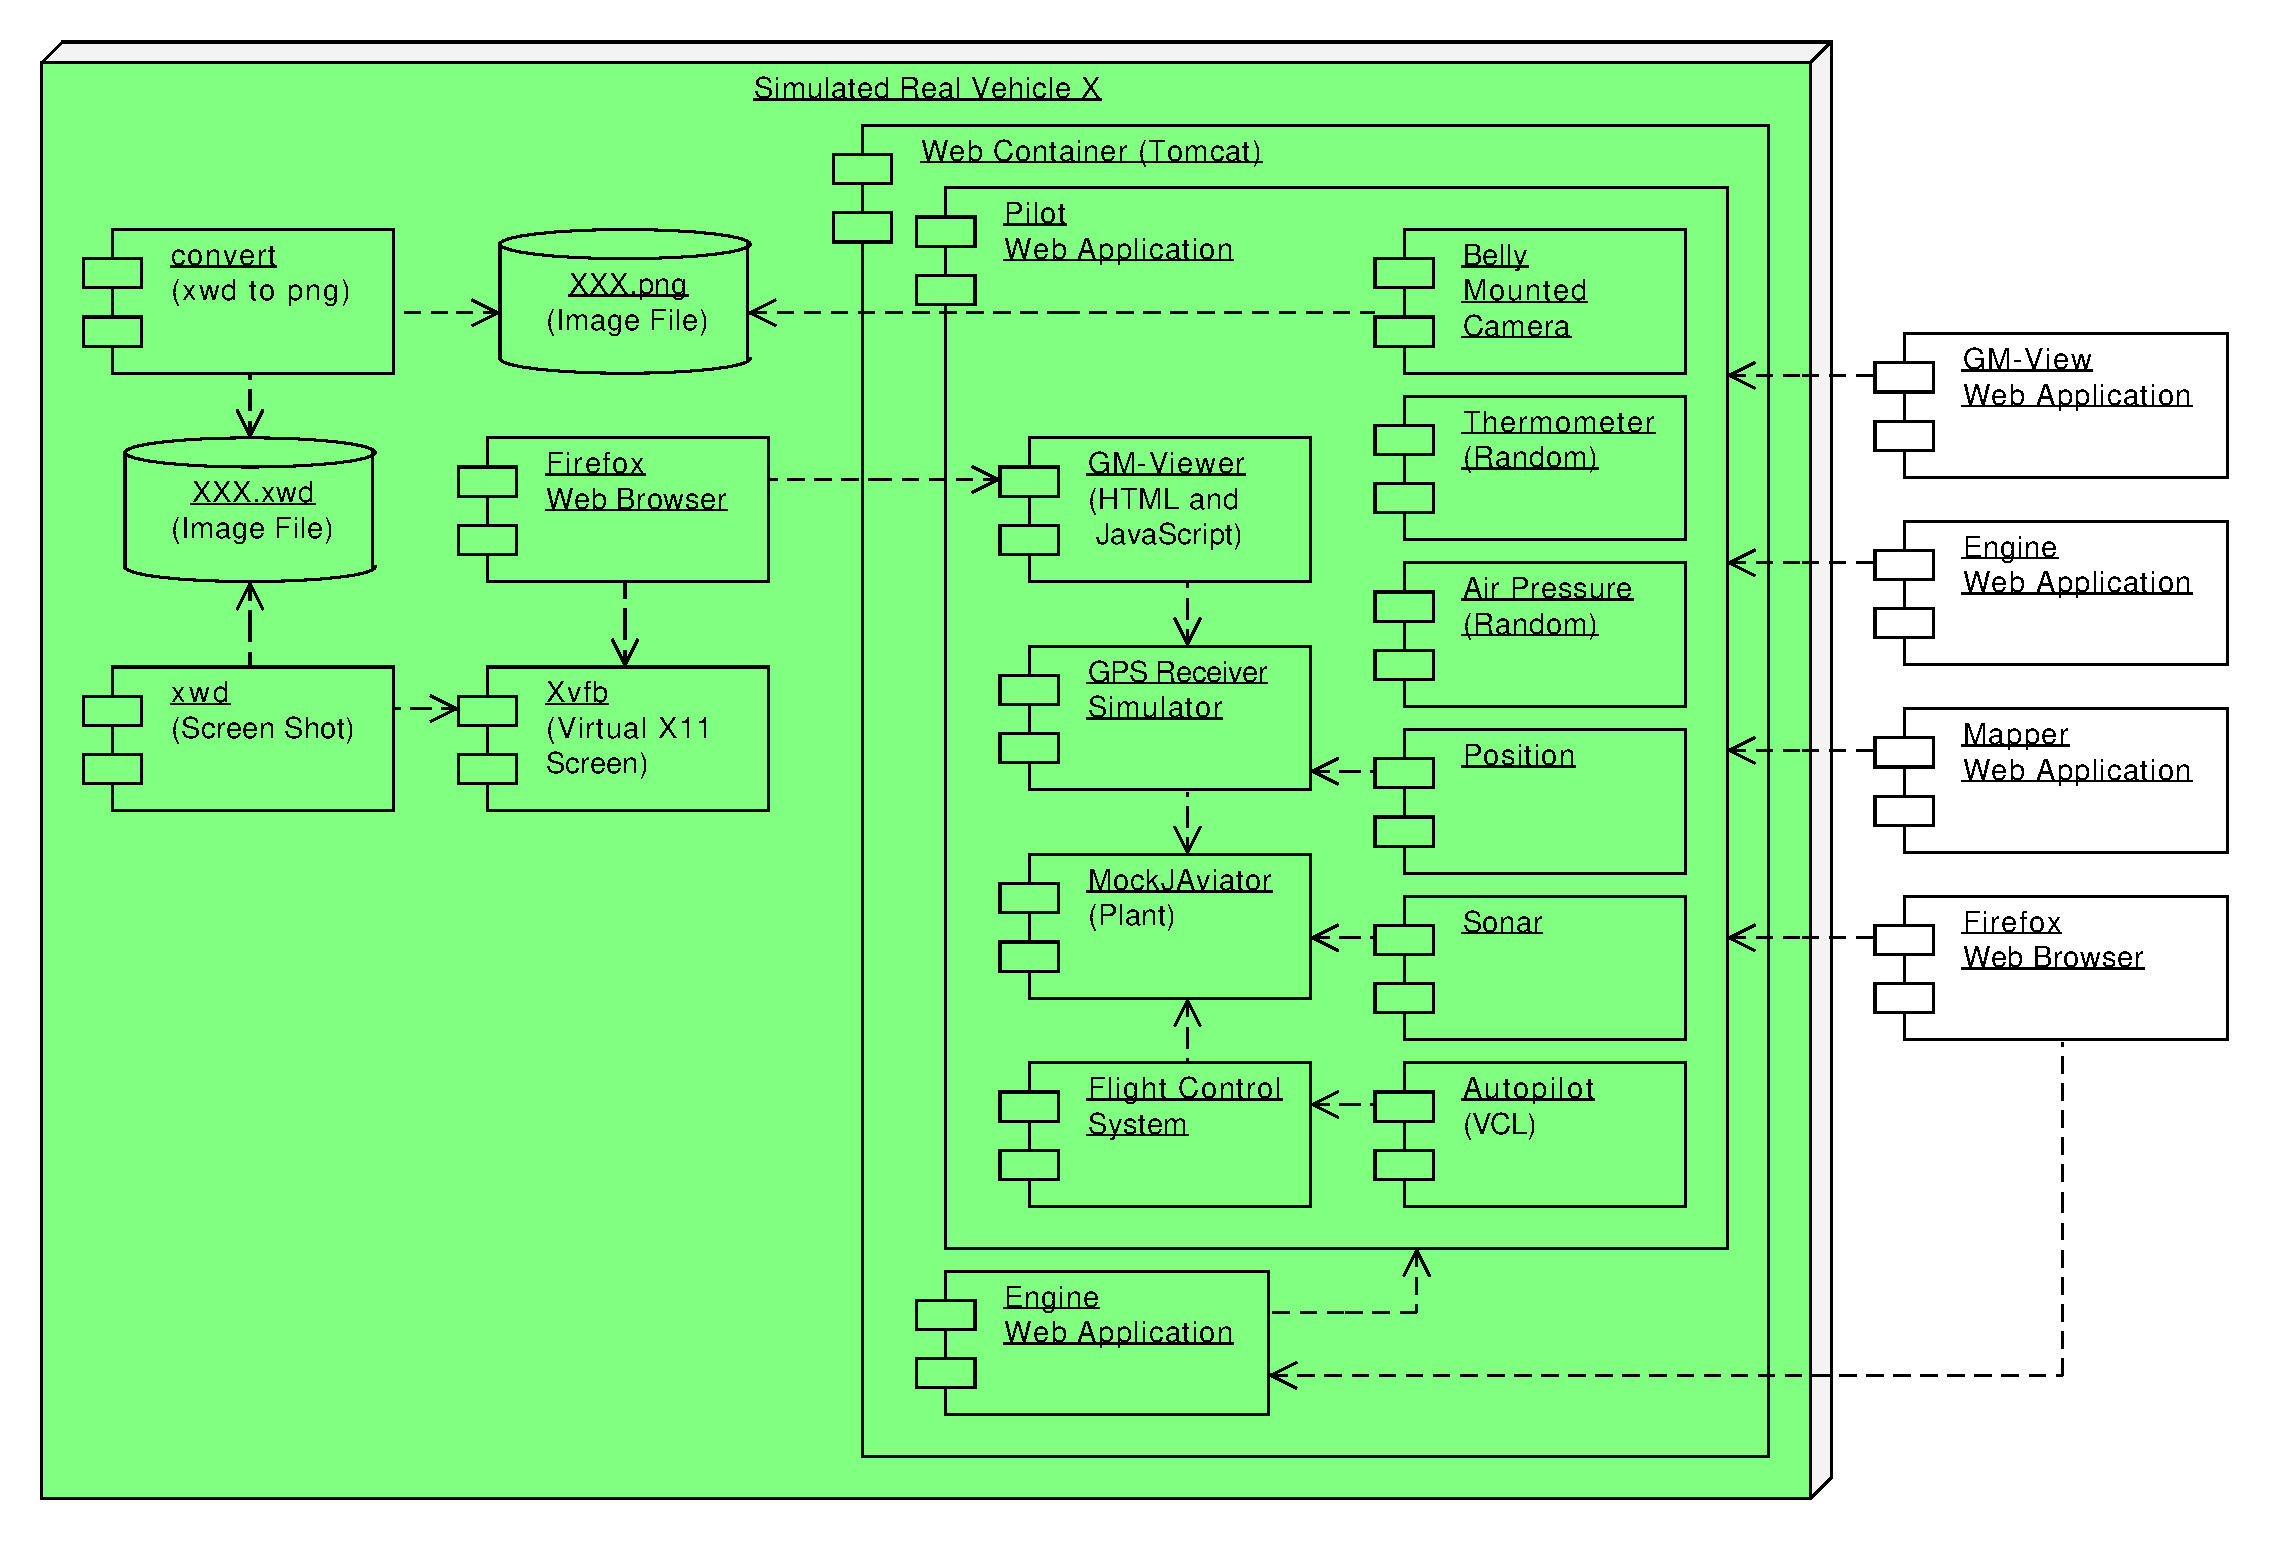
\includegraphics[width=11.6cm]{SensorSimulation-3.pdf}}
	\end{center}
	\caption{Sensor Simulation.\label{fig:SensorSimulation}}
\end{figure}


The belly mounted camera delivers a Google Maps satellite image indicating the position of the simulated vehicle by
means of a visual marker, exemplified by Figure~\ref{fig:BellyMountedCamera}.
To achieve this, the Pilot web application supplies a JavaScript enhanced HTML page.
\begin{figure}[h]
	\begin{center}
		{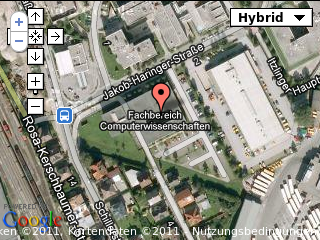
\includegraphics[width=6cm]{bmc-photo-cosy.png}}
	\end{center}
	\caption{A photo captured by the belly mounted camera.\label{fig:BellyMountedCamera}}
\end{figure}

Once the Firefox web browser selects this page, the embedded JavaScript program periodically polls the Pilot web
application for the vehicle's current position. After that, the JavaScript program slides the center of the
displayed satellite view to this position and repositions the marker.
To allow several belly mounted cameras being simulated on the same machine, the utilized web browsers use \ac{Xvfb}
devices as output screens.
%
Whenever the belly mounted camera needs to deliver a photo, it applies the \texttt{xwd} utility to take a snapshot
of the corresponding \ac{Xvfb} device, converts this snapshot to an image in PNG format by using program
\texttt{convert}, and delivers it via the \ac{HTTP}.

Thermometer and air pressure sensors apply random number generators to simulate values.
The position sensor queries the GPS receiver simulator for the current position of the vehicle, and the sonar
sensor reads the current altitude over ground from the instantiated MockJAviator.

\section{Configuration}
This section covers the configuration of the web applications Pilot, Engine, Mapper, and GM-Viewer.

\subsection{Pilot Web Application}
The configuration of the Pilot web application consists of three parts. The first part is the configuration of the
simulated model helicopter hardware, the second part is the configuration of simulated sensors, and the third
part is the assigned \ac{VCL} script.

Listing~\ref{lst:virtHWconfig} depicts a fully simulated \ac{RV}. With the property \texttt{plant.simulated} equal
to \texttt{true}, the Pilot web application simulates the model helicopter's flight dynamics of the physical body
including the \ac{IMU}.
The simulated model helicopter of type \texttt{MockJAviator} 
awaits instructions via \acs{UDP} on address \texttt{localhost} port \texttt{9011} from a controller that
operates attitude and altitude. 
\lstset{tabsize=3,language=Tex}
\begin{lstlisting}[caption={Virtual Hardware Configuration Example},mathescape=true,label=lst:virtHWconfig]{Name}
plant.simulated = true
plant.type = MockJAviator
plant.listener = udp://localhost:9011
plant.location.system.type = gpssim
plant.location.system.listener = tcp://localhost:9012
plant.location.system.update.rate = 10

controller.simulated = true
controller.type = JControl

pilot.type = JPilot
pilot.name = Pilot One
pilot.controller.connector = udp://localhost:9014
\end{lstlisting}
The simulated model helicopter has a simulated GPS receiver onboard, which listens on \texttt{localhost} port
\texttt{9012} for \acs{TCP} clients. It delivers the vehicle positions at a rate of 10 updates per second.  

In the configuration, shown in Listing~\ref{lst:virtHWconfig}, the
Pilot web application also emulates the controller for operating attitude and altitude. The controller uses
the property \texttt{plant.location.system.listener} to determine how to access the helicopter plant, and
uses the property \texttt{pilot.controller.connector} to identify the parameters for configuring a connection
for incoming commands.

The properties prefixed by \texttt{pilot} show the type and name of the autopilot component, as well as
define the connection to the attitude and altitude controller.

Listing~\ref{lst:virtSensorConfig} depicts the configuration of simulated sensors. Property \texttt{sensor.list}
defines the sensors to be simulated. The names in this list prepended by \texttt{sensor} are part of the 
configuration that follows.
\lstset{tabsize=3,language=Tex}
\begin{lstlisting}[caption={Sensor Configuration Example},mathescape=true,label=lst:virtSensorConfig]{Name}
sensor.list = gps, sonar, temp, photo

sensor.gps.name = GPS receiver
sensor.gps.path = position
sensor.gps.uri = gps:///

sensor.sonar.name = Sonar
sensor.sonar.path = sonar
sensor.sonar.uri = sonar:///

sensor.temp.name = Thermometer
sensor.temp.path = temperature
sensor.temp.uri = rand:///18/22
sensor.temp.precision = 1

sensor.photo.name = Belly Mounted Photo Camera
sensor.photo.path = photo
sensor.photo.uri = x11:///:21
sensor.photo.type = snapshot
\end{lstlisting}
Each sensor configuration defines a \texttt{name}, a \texttt{path}, and an \texttt{uri} parameter.
The parameter \texttt{name} of a sensor simply indicates its name, which is used for visualization only.
The parameter \texttt{path} is a suffix to an \acs{URL} dependent on the deployment context of the corresponding
Pilot web application. Let's assume, for example, the Pilot web application is deployed in a
web container's context \texttt{/pilot} listening on machine \texttt{nanook} port \texttt{9010}.
To access the Pilot web application, an operator uses the \acs{URL} \texttt{http://nanook:9010/pilot}. In this
example the \acs{URL} to access the above configured belly mounted photo camera is
\texttt{http://nanook:9010/pilot/sensor/photo}. 

GPS receiver and sonar sensor only have the protocol part of their \acs{URI} specified to indicate their data source.
The thermometer utilizes a random number generator to simulate values between \unit{18}{\celsius} and
\unit{22}{\celsius} providing a precision of one decimal digit.  
The belly mounted photo camera captures snapshots of the X11 screen identified by display number 21.

Listing~\ref{lst:VclExample} illustrates a \ac{VCL} script example. 
The character \texttt{\#} indicates lines containing comments.
%
The first command in this example, ``\texttt{go auto}'', switches the vehicle into autopilot mode. Without
this command, all following commands are ignored. Command ``\texttt{takeoff}'' starts the vehicle's engines
and lifts it off the ground to an altitude of \unit{1}{\meter} within \unit{5}{\second}.
%
The ``\texttt{fly to}'' commands define waypoints the vehicle has to traverse by specifying latitude, longitude,
and altitude above ground in absolute values. Additionally, this commands define a certain precision to
determine when a waypoint has been reached, e.g., a sphere of \unit{1}{\meter} radius. Furthermore, this commands
assign an average velocity to approach waypoints, e.g., \unit{2}{\meter\per\second}.
% 
\lstset{tabsize=3,language=Tex}
\begin{lstlisting}[caption={Vehicle Control Language Example},mathescape=true,label=lst:VclExample]{Name}
##
## @(#) real vehicle set course example
##
go auto
takeoff 1m for 5s
fly to (47.82204197, 13.04086670, 20)abs precision 1m 2mps
fly to (47.82206088, 13.04092035, 20)abs precision 1m 2mps
fly to (47.82195102, 13.04488063, 20)abs precision 1m 2mps
hover for 20s
land
go manual
\end{lstlisting}
%
As soon as all waypoints have been traversed, command ``\texttt{hover}'' instructs the vehicle to hold its
position at the last waypoint for, in this example, \unit{20}{\second}. After that, command ``\texttt{land}''
directs the vehicle to land. Finally, command ``\texttt{go manual}'' switches back to manual control.


\subsection{Engine Web Application}

As depicted in Listing~\ref{lst:engineConfig}, the Engine web application configuration consists
of two parameters. Parameter \texttt{pilot.url} specifies the Pilot web application the Engine
travels with, and parameter \texttt{mapper.registry.url} defines the Mapper registry service to
register with.
\lstset{tabsize=3,language=Tex}
\begin{lstlisting}[caption={Engine Configuration Example},mathescape=true,label=lst:engineConfig]{Name}
pilot.url = http://localhost:9010/pilot
mapper.registry.url = http://localhost:9040/mapper/registry
\end{lstlisting}



\subsection{Mapper Web Application}
Since every Engine web application registers with the Mapper, the Mapper web application needs no
configuration parameters. The selection of mapping algorithms is built-in and not for configuration yet.



\subsection{GM-Viewer Web Application}
Currently, the Google Maps Viewer web application needs to know every Pilot web application
and every Engine web application. As shown in Listing~\ref{lst:gmViewerConfig}, the \acs{JSON} \cite{RFC_4627}
query service \acsp{URL} for the current position, the set course's list of waypoints, and the  
list of currently assigned vehicles have to be configured for each \ac{RV} carrying a Pilot and an Engine.   

\lstset{tabsize=3,language=Tex}
\begin{lstlisting}[caption={Google Maps Viewer Configuration Example},mathescape=true,label=lst:gmViewerConfig]{Name}
pilot.list = one, two

pilot.one.name = Pilot One
pilot.one.position.url = \
	http://localhost:9010/pilot/json/position
pilot.one.waypoints.url = \
	http://localhost:9010/pilot/json/waypoints
pilot.one.vehicle.status.url = \
	http://localhost:9010/engine/json/vehicle

pilot.two.name = Pilot Two
pilot.two.position.url = \
	http://localhost:9020/pilot/json/position
pilot.two.waypoints.url = \
	http://localhost:9020/pilot/json/waypoints
pilot.two.vehicle.status.url = \
	http://localhost:9020/engine/json/vehicle
\end{lstlisting}





\section{Vehicle Virtualization}

%VV intro
A \acf{VV} is a software implementation providing an isolated environment to the end user of the service. \acp{VV} are
hosted on \acfp{RV} and offer an abstracted interface to the host's functionality. It should be possible for the end
user to specify the behavior of \acp{VV} and the jobs that should be executed by them.

\subsection{Virtual Vehicle Programming Language}

%VV language
For abstraction of services to end users a dedicated \ac{VV} programming language has been defined. The language
is targeted to be simple in usage. Listing~\ref{lst:vvProgram} shows a program example. The program represents a
list of commands. Each command consists of a point and a list of actions that have to be executed at this point. The
point definition contains the geographic location (latitude, longitude, altitude) and the specification of a tolerance
radius. The tolerance radius defines a sphere around the point in which the actions have to be performed.

\lstset{tabsize=3,language=Tex}
\begin{lstlisting}[caption={Virtual Vehicle Sample Program},mathescape=true,label=lst:vvProgram]{Name}
Point 47.82201946 13.04082647 1.00 tolerance 12.3
Picture
Temperature

Point 47.82203026 13.04084659 25.00 tolerance 100
Temperature

Point 47.82211311 13.04076076 30.00 tolerance 1.2
Picture
\end{lstlisting}

\subsection{Parsing Virtual Vehicle Programs}
When a \ac{VV} is activated the program file is read and parsed. The implemented scanner allows extending the 
language by adding control structures like ``\texttt{if~(\ldots)~else}'' or ``\texttt{for~(\ldots)}'' loops. Keywords
can be added easily and parsing of doubles, integers, and identifier is already implemented. 
%
Parsing is done based on on the EBNF specification shown in Listing~\ref{lst:vvEBNF}.

\lstset{tabsize=3,language=Tex}
\begin{lstlisting}[caption={Virtual Vehicle EBNF},mathescape=true,label=lst:vvEBNF]{Name}
Command = Position Action-List
Position = Point Tolerance
Point = "Point" double double double
Tolerance = "Tolerance" double
Action-List = Action {Action}
Action = "Temperature" | "Picture" | "Airpressure" |
	"Altitude" | "Speed"
\end{lstlisting}


%If an error occurs during the parsing of the program file an exception is thrown. With the exception and detailed error
% description is provided. Parsing is stopped and the rest of the file ignored.
%If the file was successfully parsed then the parser returns a list of command objects.
%Each of this objects include a position object and a list of actions.

If an error occurs during program parsing, the parser stops and throws an exception. For easier debugging, the exception
contains a detailed error description. If the parser succeeds parsing the program, it returns a list of command objects.
Each of this objects contains a position and a list of actions.
A position includes a point with a tolerance as described above.

\subsection{Executing Virtual Vehicle Programs}

A \ac{RV} can host one or more \ac{VV}. Each \acp{VV} executes in a separate thread.
When a \ac{VV} is scheduled the first time, it takes the first command from its command list, which was
returned from the parser, and starts executing this command. A command can be executed if the position of the \ac{RV} is
within the tolerance sphere specified in its position, that means, the actions, like taking a picture, measuring the
temperature, etc., can be performed.
If it's not possible to finish a command, because of a wrong position or actions can not be done, the \ac{VV} keeps
active.


\subsection{Migration}

\acp{VV} have the ability to suspend while they are executing their job. In this mode the entire internal state 
information is persisted to a file. While being in the suspended state it is possible to migrate the \ac{VV} to another
\ac{RV} host and resume the operation there. To store the state the Java serialization is used. The whole command
list is serialized to a file, that means the already finished commands and the command that have to be executed are
written to disk. The results of the executed actions are stored in different files. After migration when the state is
read back, the \ac{VV} looks at the command list and begins again to execute commands. All commands which are already
executed are skipped. The \ac{VV} continues with the first unfinished command. Unfinished could also mean that some of
the actions where already executed.


\subsection{Types of Mobility}
The migration process is denominated as \emph{cyber mobility}, because no real vehicle movement is taking place when a
\ac{VV} changes its location. Movements that are carried out on board of a not changing \ac{RV} host
are known as \emph{physical mobility}.

Each \ac{VV} records its movements. This historical track is represented by a list of waypoints. Each waypoint
contains a timestamp, the geographic location and the name of the host. The host name is necessary to differ between
cyber mobility and physical mobility. Waypoints are stored when a \ac{VV} executes a cycle and its location has
changed more than a specific distance (physical mobility) or its host has changed (cyber mobility). With the information
that is stored in the track detailed analysis of \ac{VV} moving behavior will be possible, which means that there is
no way to access this data by now.



\section{Mapping}
The Mapper is responsible for automatically mapping \acp{VV} to \acp{RV}. To accomplish this, the mechanism invokes 
the migration of \acp{VV} based on a mapping decision made by a mapping algorithm.
Additionally to the Mapper itself with its mapping algorithm, a registration service is present.

The servlet stores all registration information persistent in a file, otherwise registered Engines would be lost in
a restart. This is important because only registered Engines are considered during the mapping process.

\subsection{Registration Service}
An Engine registers itself with the registration service upon start up using its ID. If the registration was successful, the service
fetches some useful information and stores it together with the Engine ID. The fetched information are available sensors
and way points (flight plan), in our case, these is static information. If a registration attempt was not successful, the
Engine keeps trying to register until it succeeds.

\subsection{Mapper}
The mapper periodically executes the following three steps: 

\begin{enumerate}
  \item Fetch the status of all \acp{VV} from all registered Engines.
  The returned message includes the current active action point, and its unfinished actions.
  
  \item Fetch the status of all \acp{RV} on which an Engine is running.
  The returned message includes the current position, the next position, and the average velocity.
  
  \item Execute the mapping algorithm.
\end{enumerate}

At the time of writing, there are two algorithms available that can be set in the configuration file: a random
mapping algorithm and a simple mapping algorithm.

\textbf{Random Mapping Algorithm}

This algorithm does not use any information concerning flight plans and available sensors.
It randomly selects two different Engines. If one of these has \acp{VV}, then it selects one of this \acp{VV}
and initiates a migration to the other Engine.

\textbf{Simple Mapping Algorithm}

Listing~\ref{lst:simpleMappingAlgorithm} reveals the simple mapping algorithm as pseudo code. 

\lstset{tabsize=3,language=PseudoCode}
\begin{lstlisting}[caption={Simple Mapping Algorithm},mathescape=true,label=lst:simpleMappingAlgorithm]{Name}
for all virtual vehicles do
	if virtual vehicle program is complete
	then
		invoke migration to central engine
	else
		find fastest real vehicle with at least one fitting
		sensor and a distance between the line Current to Next
		and ActionPoint smaller than the tolerance
	endif
	if found vehicle 
	then 
		invoke migration to it 
	endif
endfor
\end{lstlisting}

The fastest vehicle is the vehicle with the shortest flight time from its current position to the action
point of the \ac{VV}.
%(thus: higher precision \begin{math} \rightarrow \end{math} faster) of the virtual vehicle. 


Figure~\ref{fig:intersectionExample} shows the current flight path of a \ac{RV}, its current location $C$,
and the end point of the current flight plan segment $N$.
% Illustration of line segment to action point distance:
\begin{figure}[h]
	\begin{center}
		{
            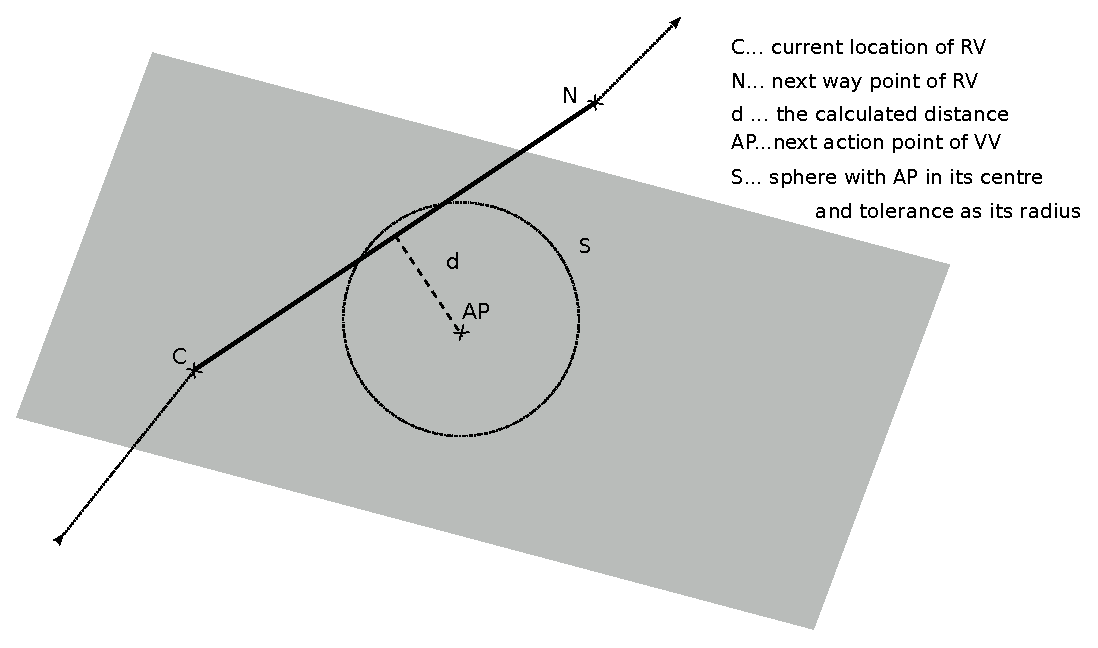
\includegraphics[width=12cm]{dist.eps}
        }
	\end{center}
	\caption{Intersection of flight path and next action point.\label{fig:intersectionExample}}
\end{figure}
% This example 
The flight path $\displaystyle{\overrightarrow{CN}}$ intersects with the tolerance sphere of action point $AP$, thus
the distance is smaller than the tolerance and the \ac{RV} is a candidate for migration. With the given speed
of the \ac{RV}, the mapping algorithm calculates the flying time of the \ac{RV} to reach action point $AP$. The
algorithm selects the \ac{RV} with the smallest flying time to reach $AP$ as a migration target for the concerned
\ac{VV}.
%
With this behavior of the algorithm, a \ac{VV} stays on a \ac{RV} or the central Engine until a \ac{RV}
enters a flight plan segment that satisfies the \ac{VV}'s sensor and location requirements.



%%
%% Results
%%

\chapter{Results}

This chapter summarizes the four demonstrations held in class on January 24, 2012. The main goal of this
demonstrations was to show data collecting \acp{VV} carried by \acp{RV}, as well as \acp{VV} migrating
among \acp{RV}. All images shown in this chapter were rendered by utilizing Google Maps \cite{GOOGLEMAPS2012} in a web browser.


\section{Demonstration 1: Data Collection}
In this demonstration one flying \ac{RV} carries one \ac{VV}, which collects data at four locations.
\begin{figure}[h]
	\begin{center}
		\begin{tabular}{cc}
			a)&{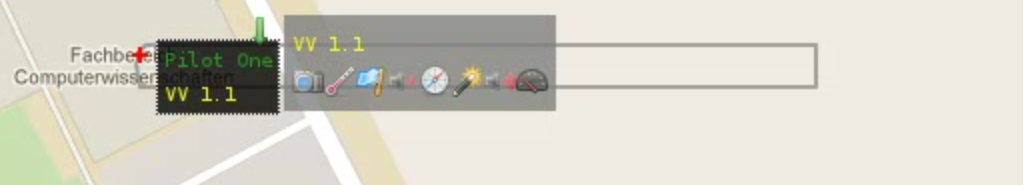
\includegraphics[width=9.4cm]{ese-demo1-1.png}} \\
			b)&{
\includegraphics[width=9.4cm]{ese-demo1-2.png}} \\
			
			c)&{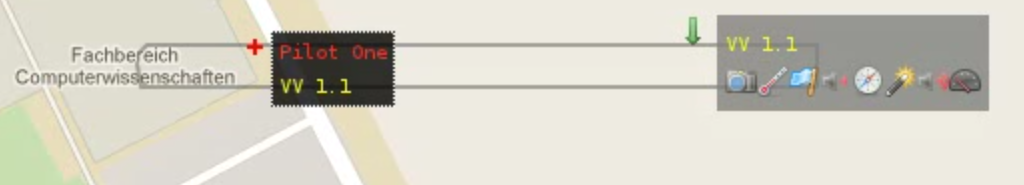
\includegraphics[width=9.4cm]{ese-demo1-3.png}} \\
			d)&{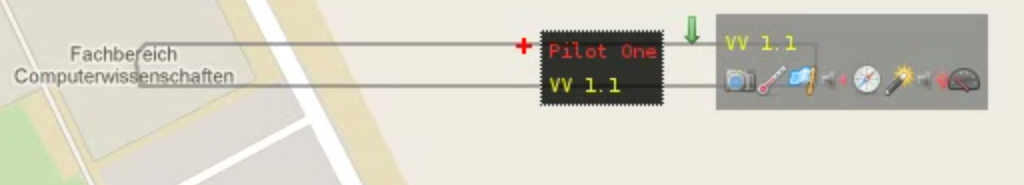
\includegraphics[width=9.4cm]{ese-demo1-4.png}} \\
			
			e)&{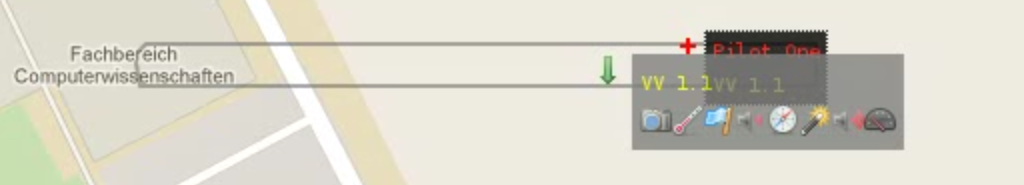
\includegraphics[width=9.4cm]{ese-demo1-5.png}} \\
			f)&{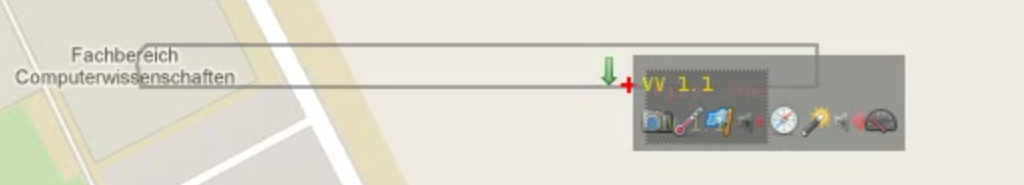
\includegraphics[width=9.4cm]{ese-demo1-6.png}} \\
	
			g)&{
\includegraphics[width=9.4cm]{ese-demo1-7.png}} \\
			h)&{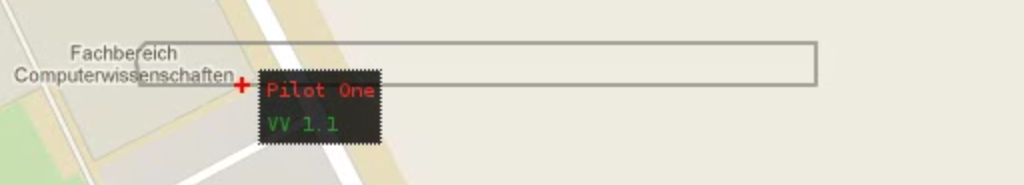
\includegraphics[width=9.4cm]{ese-demo1-8.png}}
		\end{tabular}
	\end{center}
	\caption{Data Collection Demonstration.\label{fig:demo1}}
\end{figure}
Figure~\ref{fig:demo1}~a displays \ac{RV} \textit{Pilot~One} with \ac{VV} \textit{VV~1.1} onboard.
The color green of \textit{Pilot~One} indicates that the \ac{RV} is still on the ground, and the
color yellow of \textit{VV~1.1} shows that the \ac{VV} still has action points to process.
The action points of \textit{VV~1.1} command accessing the sensors belly mounted photo camera, thermometer,
barometer, sonar, course over ground, random, GPS altitude, and speed over ground. 
In Figure~\ref{fig:demo1}~b \textit{Pilot~One} approaches the first action point. The red label indicates
that the \ac{RV} is flying. After completing the first action point \textit{Pilot~One} approaches the
second action point of \textit{VV~1.1}, as depicted in Figures~\ref{fig:demo1}~c and \ref{fig:demo1}~d.
Figures~\ref{fig:demo1}~e, \ref{fig:demo1}~f, and \ref{fig:demo1}~g visualize \textit{Pilot~One} heading
for the third and fourth action point. After processing the fourth action point, the \ac{VV}'s label
becomes green, which denotes the completion of \textit{VV~1.1}'s mission.

\section{Demonstration 2: Migration}
In this demonstration two \acp{RV} fly along their set courses and one \ac{VV} collects data at five locations.
The blue line in Figure~\ref{fig:demo2vvPath} suggests the virtual path of vehicle \textit{VV~2.1}.
\begin{figure}[h]
	\begin{center}
		{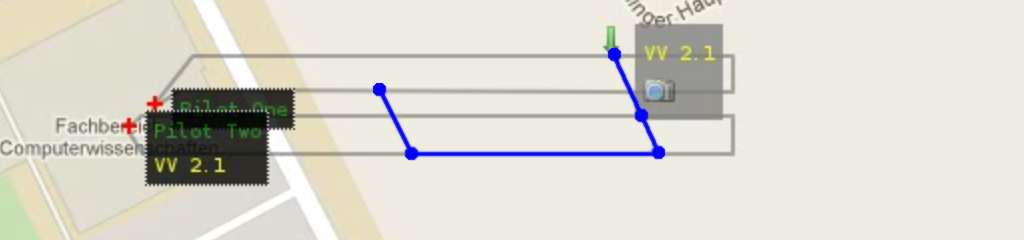
\includegraphics[width=9.4cm]{ese-demo2-1.png}}
	\end{center}
	\caption{Path of Virtual Vehicle \textit{VV~2.1}.\label{fig:demo2vvPath}}
\end{figure}
Initially, \ac{RV} \textit{Pilot~Two} carries \textit{VV~2.1}. After the \acp{RV} take off, a migration
of \textit{VV~2.1} from \textit{Pilot~Two} to \textit{Pilot~One} must take place to allow the \ac{VV} to
reach the first action point. The currently available mapping algorithm considers only the current
set course segment of a \ac{RV} for mapping decisions.
In this demonstration the first action point resides on the second segment of the  set course of
\textit{Pilot~One}. As displayed in Figure~\ref{fig:demo2mig01}, the mapper migrates \textit{VV~2.1} as
soon as \textit{Pilot~One} enters its second set course segment. 
\begin{figure}[h]
	\begin{center}
		{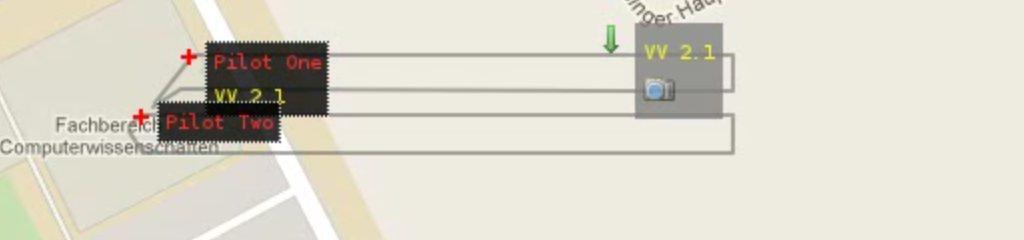
\includegraphics[width=9.4cm]{ese-demo2-2.png}}
	\end{center}
	\caption{First migration of \textit{VV~2.1} from \textit{Pilot~Two} to \textit{Pilot~One}
	initiated by a decision of the mapping algorithm.\label{fig:demo2mig01}}
\end{figure}
\textit{VV~2.1} resides on \textit{Pilot~One} until the \ac{RV} reaches the first action point
(Figure~\ref{fig:demo2mig02}~a). As soon as \textit{VV~2.1} has captured an image via the belly mounted camera,
the mapping algorithm decides to initiate a migration of the \ac{VV} to \textit{Pilot~Two}
(Figure~\ref{fig:demo2mig02}~b). Then, \textit{VV~2.1} takes a picture on the second action point.  
%
Now, there are no action points in the current set course segments of both \acp{RV}. In such a case
the currently implemented mapping algorithm can not decide whether migrating the \ac{VV} would be
beneficial or not. So, the \ac{VV} stays on board of \textit{Pilot~Two} until the mapping algorithm
decides otherwise.
%
\begin{figure}[h]
	\begin{center}
		\begin{tabular}{rr}
			a)&{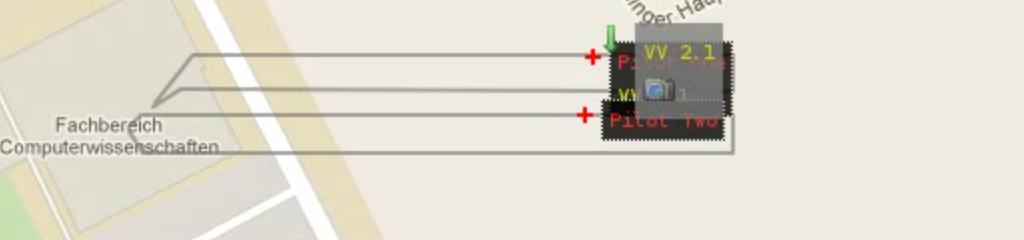
\includegraphics[width=9.4cm]{ese-demo2-3.png}} \\
			b)&{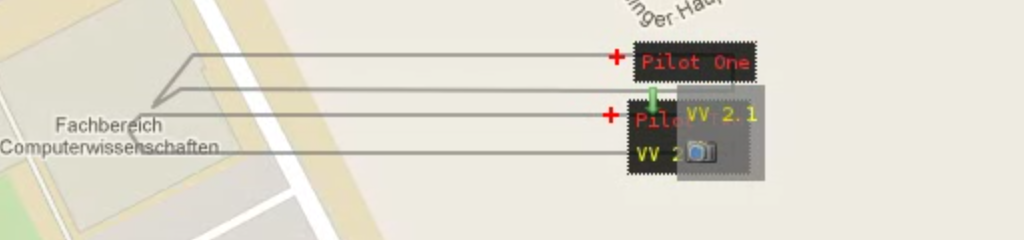
\includegraphics[width=9.4cm]{ese-demo2-4.png}} \\
			c)&{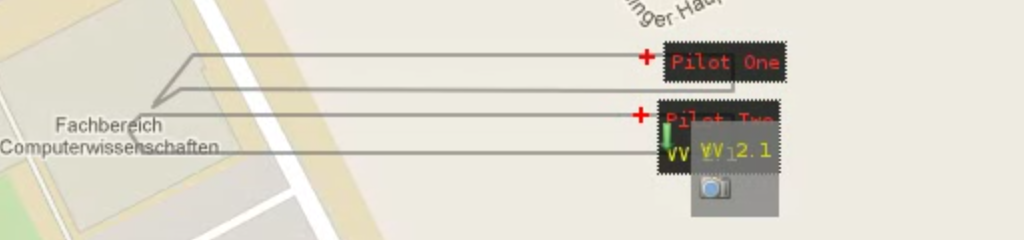
\includegraphics[width=9.4cm]{ese-demo2-5.png}} \\
			d)&{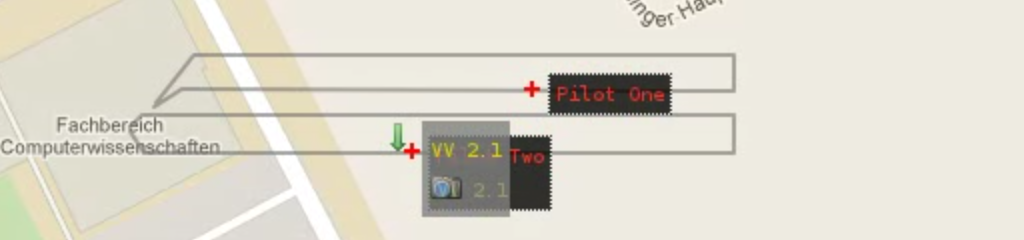
\includegraphics[width=9.4cm]{ese-demo2-6.png}} \\
			e)&{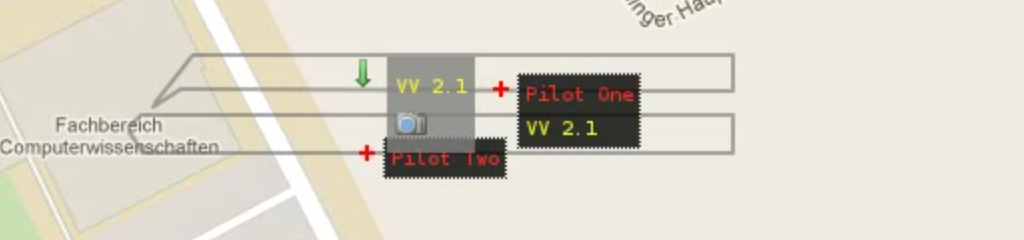
\includegraphics[width=9.4cm]{ese-demo2-7.png}} \\
			f)&{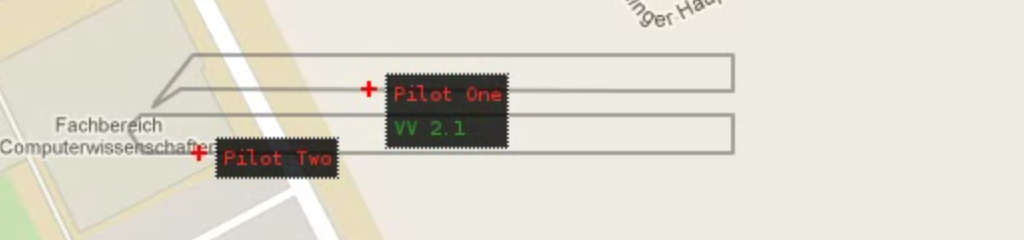
\includegraphics[width=9.4cm]{ese-demo2-8.png}}
		\end{tabular}
	\end{center}
	\caption{\textit{Pilot~One} and \textit{Pilot~Two} mutually carrying \textit{VV~2.1}
		caused by migration decisions of the mapping algorithm.\label{fig:demo2mig02}}
\end{figure}
The \acp{RV} continue to traverse their set courses until \textit{Pilot~Two} enters the fourth segment.
The mapping algorithm detects that \textit{VV~2.1} already is onboard \textit{Pilot~Two} and suppresses
a migration. In Figures~\ref{fig:demo2mig02}~c and \ref{fig:demo2mig02}~d \textit{VV~2.1} captures
photos at the third and at the fourth action point.
%
For the fifth action point, the mapping algorithm decides a migration of \textit{VV~2.1} back to
\textit{Pilot~One}, as visualized in Figure~\ref{fig:demo2mig02}~e. After taking a picture at the last
action point, \textit{VV~2.1} has completed its mission. To indicate this, the label of \textit{VV~2.1}
turns green (Figure~\ref{fig:demo2mig02}~f).
Finally, the mapping algorithm decides a migration back to the central Engine.


\section{Demonstration 3: Different Sensors}
The \acp{RV} in this demonstration do not have the same set of sensors. The first \ac{RV}, \textit{Pilot~One},
carries a thermometer, the second \ac{RV}, \textit{Pilot~Two}, ferries a barometer, and the third \ac{RV},
\textit{Pilot~Three}, transports a belly mounted camera.
All three \acp{RV} follow the same set course in sequence and keep a flying distance of \unit{10}{\second}.
The task list of \textit{VV~3.1} consists of two action points, which require capturing photos, temperature
values, and air pressure values.   

Figure~\ref{fig:demo3mig03}~a shows all three \acp{RV} approaching the first action point. Since
\textit{Pilot~One} arrives first and provides a required thermometer sensor, the mapper algorithm already
initiated a migration of \textit{VV~3.1} to \textit{Pilot~One}. 
%
At this point in time, the indicator of the first action point visualizes all three required actions
as incomplete.
%
After \textit{VV~3.1} has completed the temperature measurement, \textit{Pilot~Two} is the next in line
to reach the action point supplying a fitting sensor. Therefore, the mapping algorithm commands a migration 
to \textit{Pilot~Two}.
%
As shown in Figure~\ref{fig:demo3mig03}~b, the action point indicator no more views
the thermometer.
\begin{figure}[h]
	\begin{center}
		\begin{tabular}{rr}
			a)&{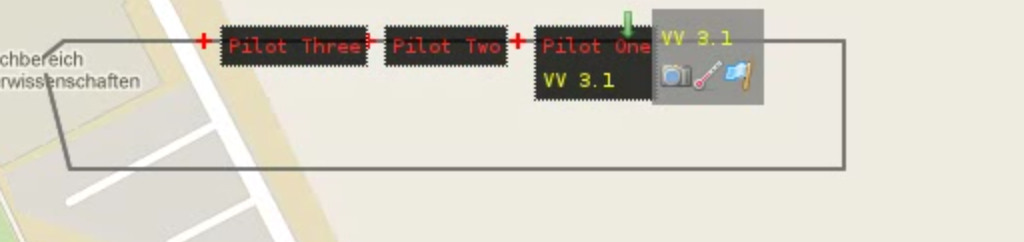
\includegraphics[width=9.4cm]{ese-demo3-1.png}} \\
			b)&{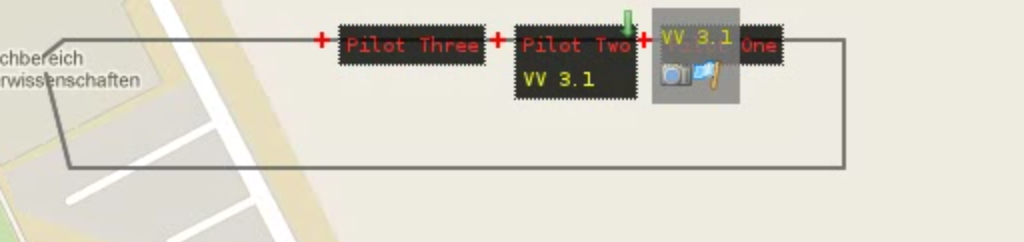
\includegraphics[width=9.4cm]{ese-demo3-2.png}} \\
			c)&{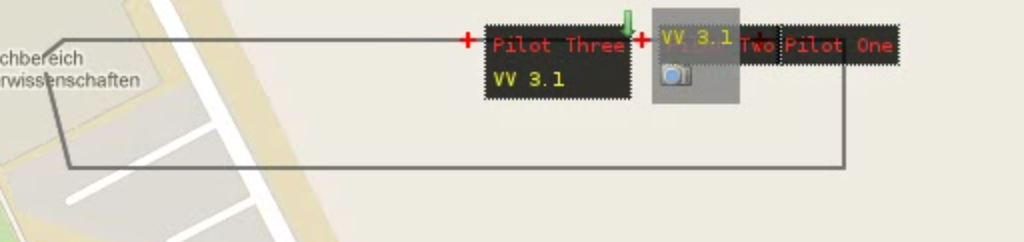
\includegraphics[width=9.4cm]{ese-demo3-3.png}} \\
			d)&{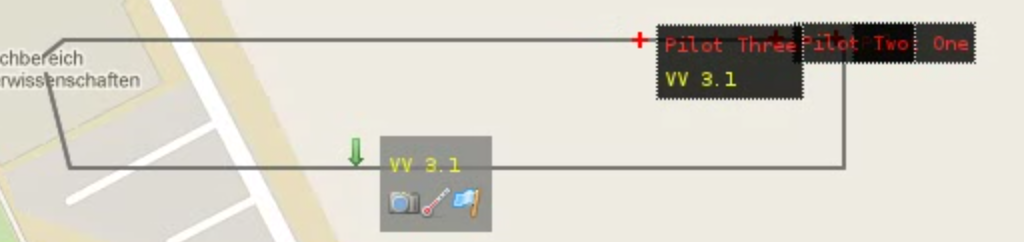
\includegraphics[width=9.4cm]{ese-demo3-4.png}}
		\end{tabular}
	\end{center}
	\caption{\acp{RV} \textit{Pilot~One}, \textit{Pilot~Two}, and \textit{Pilot~Three} mutually carrying
	 	\textit{VV~3.1} repeatedly to the first action point caused by migration decisions of the mapping
	 algorithm.\label{fig:demo3mig03}}
\end{figure}

Figure~\ref{fig:demo3mig03}~c presents the situation after \textit{VV~3.1} has measured the air pressure.
The mapper algorithm already ordered a migration of \textit{VV~3.1} to \textit{Pilot~Three} and
the action point indicator views the remaining action for taking a photo. 
%
Then, \textit{VV~3.1} stays onboard of \textit{Pilot~Three}, because the mapping algorithm can not find
a eligible \ac{RV} for processing the next action point. 

In Figure~\ref{fig:demo3mig04}~a \textit{Pilot~One} enters a set course segment that leads to the next
action point. Since \textit{Pilot~One} facilitates an adequate sensor and is the first to reach the action
point, the mapper algorithm directs a migration of \textit{VV~3.1} to \textit{Pilot~One}.

As \textit{Pilot~One} catches the action point, \textit{VV~3.1} queries the thermometer and the mapper
algorithm orders a migration to \textit{Pilot~Two} (Figure~\ref{fig:demo3mig04}~b).
Again, the action point indicator no more views the thermometer.

\begin{figure}[h]
	\begin{center}
		\begin{tabular}{rr}
			a)&{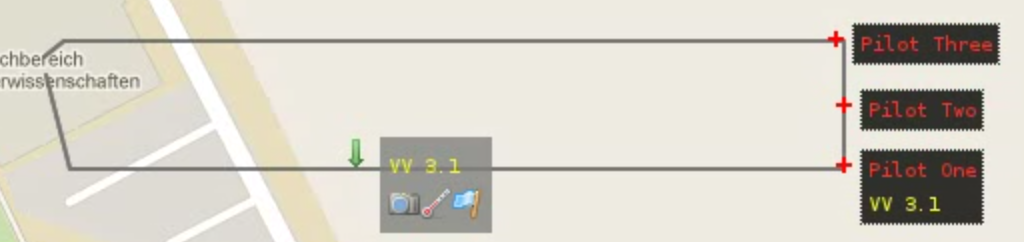
\includegraphics[width=9.4cm]{ese-demo3-5.png}} \\
			b)&{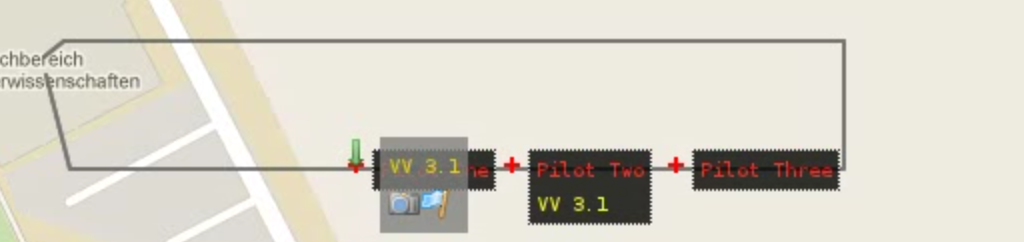
\includegraphics[width=9.4cm]{ese-demo3-6.png}} \\
			c)&{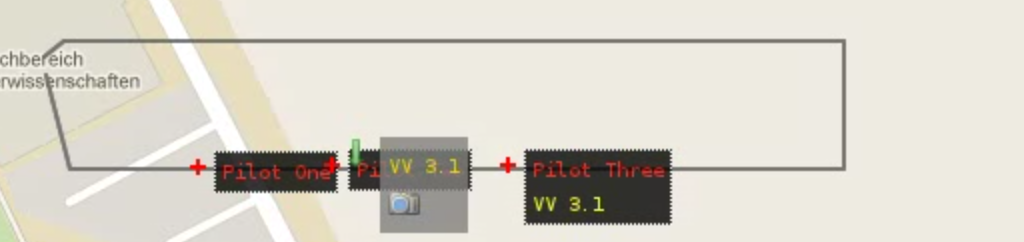
\includegraphics[width=9.4cm]{ese-demo3-7.png}} \\
			d)&{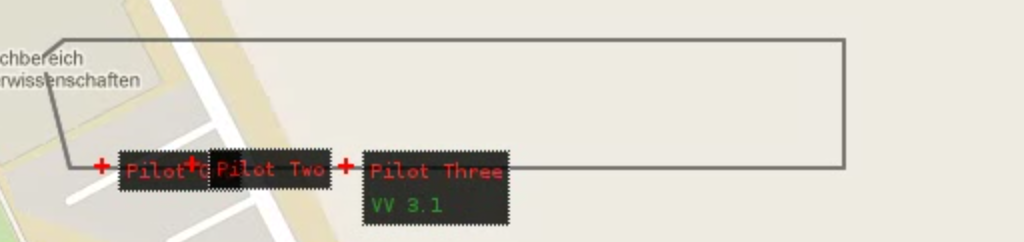
\includegraphics[width=9.4cm]{ese-demo3-8.png}}
		\end{tabular}
	\end{center}
	\caption{\acp{RV} \textit{Pilot~One}, \textit{Pilot~Two}, and \textit{Pilot~Three} mutually carrying
		\textit{VV~3.1} repeatedly to the second action point caused by migration decisions of the mapping
		algorithm.\label{fig:demo3mig04}}
\end{figure}
After that, \textit{Pilot~Two}
arrives at the action point, \textit{VV~3.1} measures the air pressure and the mapper algorithm commands
a migration to \textit{Pilot~Three} (Figure~\ref{fig:demo3mig04}~c).
Consequently, the air pressure symbol vanishes from the action point indicator.
%
Now, \textit{Pilot~Three} gets to the action point and \textit{VV~3.1} completes its mission by 
taking a picture, as shown in Figure~\ref{fig:demo3mig04}~d. The \ac{VV}'s label turns green to show this.
%
At last, the mapping algorithm initiates a migration back to the central Engine.


\section{Demonstration 4: Multiple Virtual Vehicles}
In this demonstration three \acp{RV} fly along their set courses and four \acp{VV} collect data at several locations.
Each \ac{RV} provides the same set of sensors. Initially, the \acp{VV} idle on the central Engine and wait for
the mapping algorithm to assign an eligible \ac{RV}.  
%
The blue lines in Figure~\ref{fig:demo4img1}~a display the virtual paths of the \acp{VV}.
All \ac{VV} paths progress top-down, as indicated by black arrows.

Figure~\ref{fig:demo4img1}~b shows an advanced stage of this demonstration mission displaying all four \acp{VV} in
action.
% \begin{figure}[h]
% 	\begin{center}
% 		a) {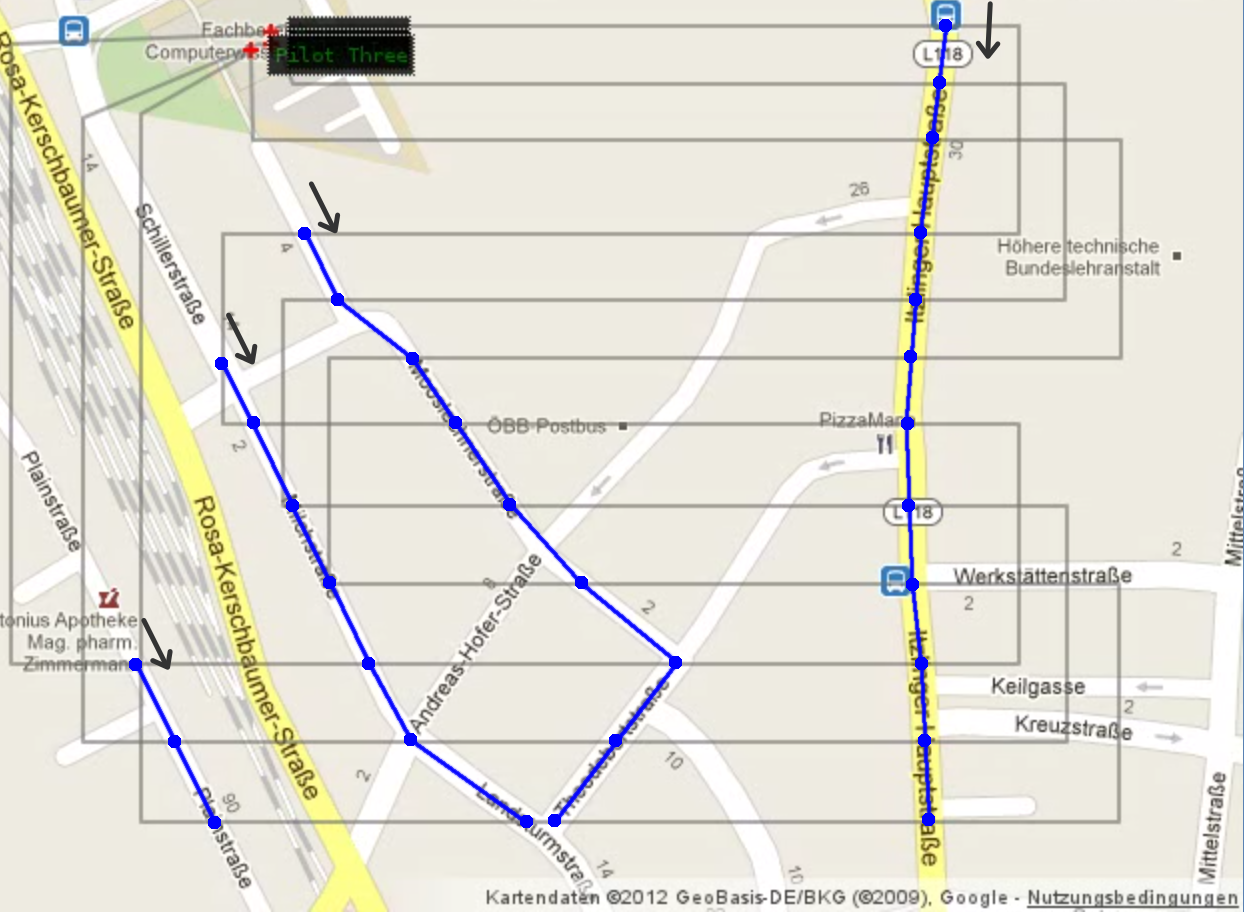
\includegraphics[width=11.1cm]{ese-demo4-1.png}}
% 	\end{center}
% 		\caption{Demonstration 4: Virtual Vehicle Paths.\label{fig:demo4img1}}
% \end{figure}
%
\begin{figure}[h]
	\begin{center}
		\begin{tabular}{rr}
		a)&{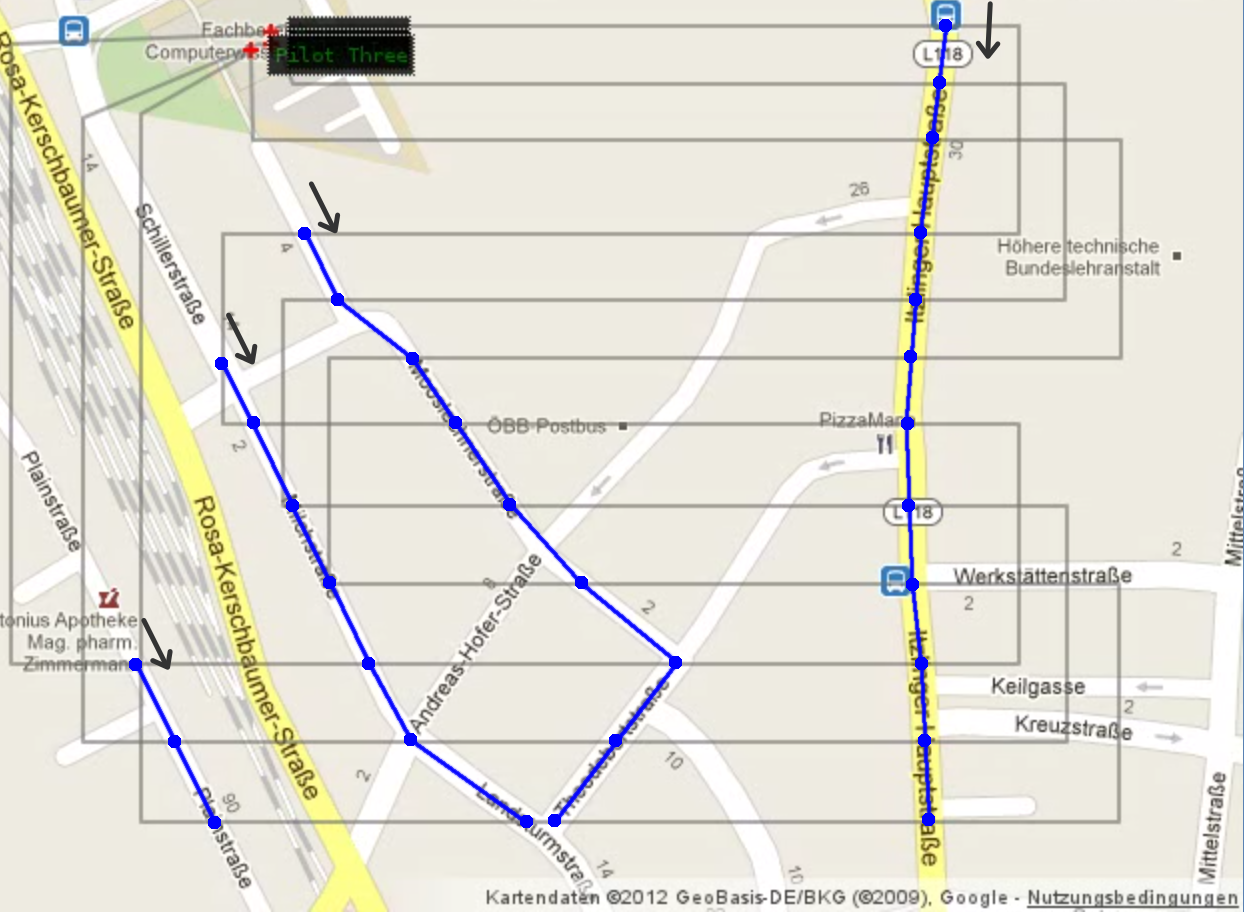
\includegraphics[width=11.42cm]{ese-demo4-1.png}} \\
		b)&{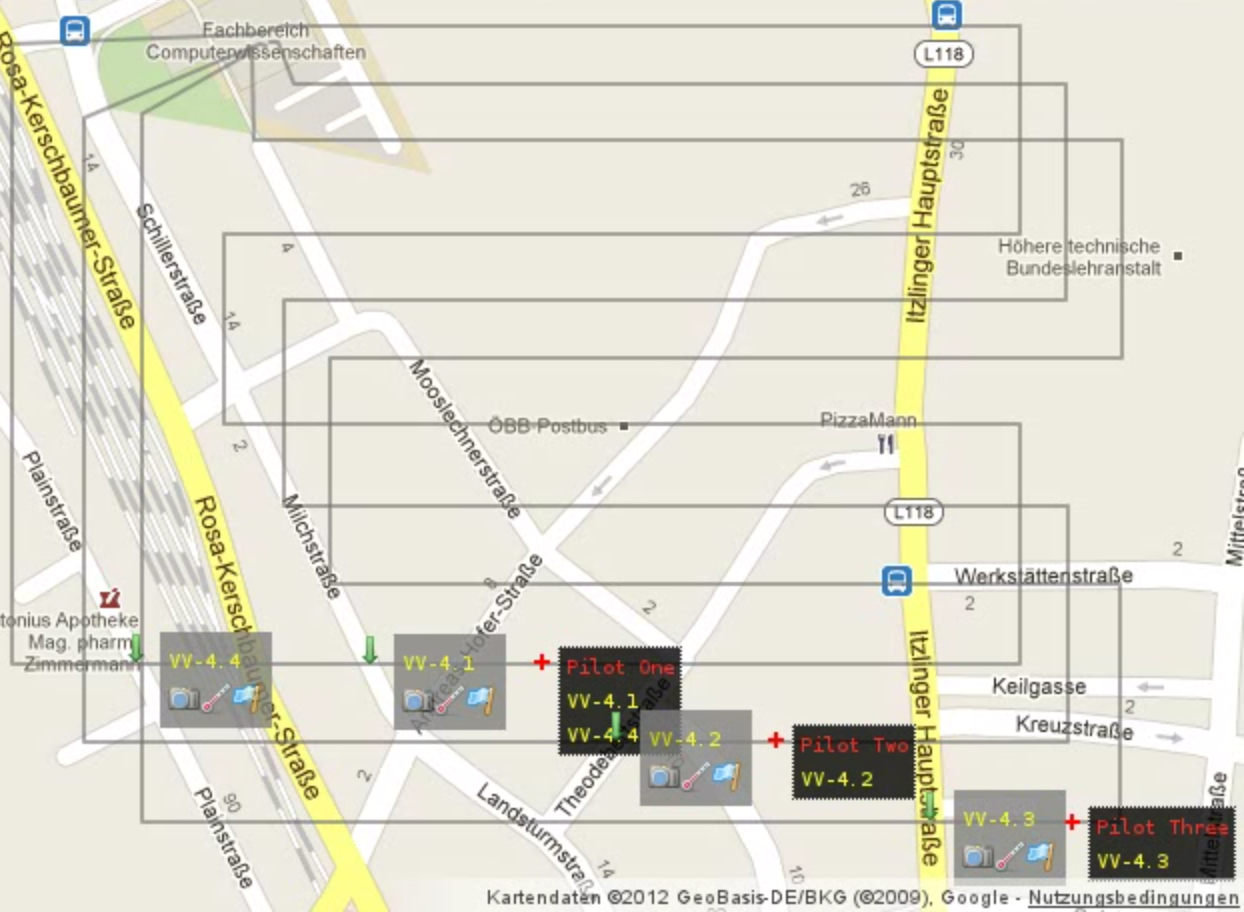
\includegraphics[width=11.42cm]{ese-demo4-2.png}}
		\end{tabular}
	\end{center}
		\caption{Demonstration 4: a) Virtual Vehicle Paths. 
		b) Multiple \acsp{VV} in action.\label{fig:demo4img1}}
\end{figure}


%%
%% Conclusion
%%

\chapter{Conclusion}

\section{Section}

\subsection{Subtitle}

Plain text.

\subsection{Another subtitle}

More plain text.



\bibliographystyle{references}
\bibliography{references}
\vfill\newpage

\chapter*{List of Abbreviations\markboth{List of abbreviations}{List of abbreviations}}
\addcontentsline{toc}{chapter}{List of abbreviations}
\thispagestyle{plain}
%%
%% Abbreviations
%%

\begin{acronym}
	\acro{CPCC}{cyber-physical cloud computing}
	\acro{HTTP}{Hyper Text Transport Protocol}
	\acro{IMU}{Inertial Measurement Unit}
	\acro{JSON}{JavaScript Object Notation}
	\acro{RV}{Real Vehicle}
	\acro{TCP}{Transmission Control Protocol}
	\acro{UAV}{Unmanned Aerial Vehicle}
	\acro{UDP}{User Datagram Protocol}
	\acro{URL}{Unified Resource Locator}
	\acro{URI}{Unified Resource Identifier}
	\acro{VCL}{Vehicle Control Language}
	\acro{VV}{Virtual Vehicle}
	\acro{VV RTE}{Virtual Vehicle Runtime Environment}
	\acro{Xvfb}{X11 virtual frame buffer}
\end{acronym}



\vfill\newpage


\end{document}
